\documentclass[12pt]{article}
\usepackage[utf8]{inputenc}
\usepackage{hyperref}
\usepackage{graphicx}

\title{Design Thinking in Human-Centered Design}
\author{Shaan Fulton}
\date{\today}

\begin{document}

\maketitle

How do we design to meet human needs? What process is most likely to create designs that solve human problems?

Perhaps we might first ask: Why solve humans needs? Design does not need to be human-centered. We can focus on other concerns: aesthetics, technological display, etc. I leave this question as an exercise to the reader.

\section*{Solving Real Problems}

If the goal of human-centered design is to solve problems, we must first identify real problems. Please observe the distinction: there are problems, and then there are \textit{real problems}. Real problems are the underlying issues that cause human dissatisfaction.

Consider the following example:

\begin{quote}
A company is trying to put water on the blockchain. They encounter a problem: Users are having trouble setting up their WaterCoin wallets, making it hard to buy water for personal use. These users have never used a crypto wallet before. A designer is tasked with making a custom wallet for the company that is easier to set up for these new users.
\end{quote}

The users are clearly dissatisfied. How can we solve this problem? A bad designer would create a more seamless custom wallet. A good designer would short the stock and run as far away as possible. Good human-centered design starts with solving real problems. The real problem here doesn't actually exist. You are solving a problem of your own creation, thus the best approach is to create nothing in the first place.

Design therefore involves both discovery of the problem as well as discovery of the solution. We model this using the \textit{double-diamond design process model}.

\begin{figure}[htbp]
\centering
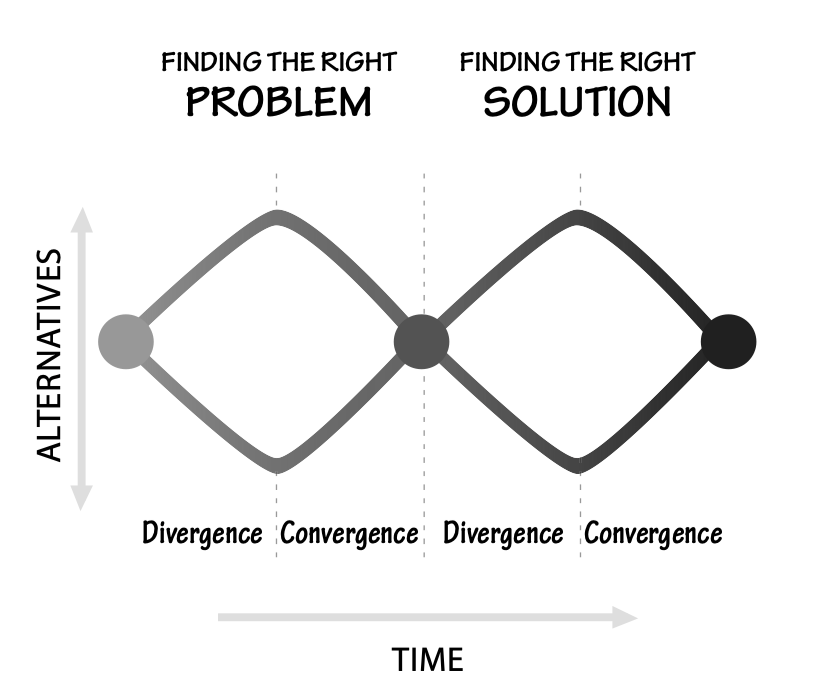
\includegraphics[width=0.8\textwidth]{diamond.png}
\caption{The double-diamond model of design}
\end{figure}

The process proceeds as follows:

\begin{enumerate}
\item A divergent problem phase in which we brainstorm many possible underlying issues, performing contextual inquiry and user research
\item A convergent problem phase in which we hone in on a few core issues
\item A divergent solution phase in which we brainstorm possible solutions for our core issues
\item A convergent solution phase in which we hone in on a few promising solutions
\end{enumerate}

So we simply figure out the core problems, and then hone in on a beautiful solution, handing it immediately off to our customers.

\section*{Working in Cycles}

There's one issue. Do you see it? \textbf{The only interaction we had with our customers was during the problem phase}. The solution phase occurs entirely in our minds. Therefore, our final solution is untested. It may not actually be optimal. We may discover a whole suite of new problems upon testing it. This is especially problematic if it is already extensively refined and changes would be costly. 

Therefore, we refine this process by making it cyclical. The non-cyclical version is what we call \textit{waterfall}. The cyclical version, especially in the context of software development, is what we call \textit{agile}.

\begin{figure}[htbp]
  \centering
  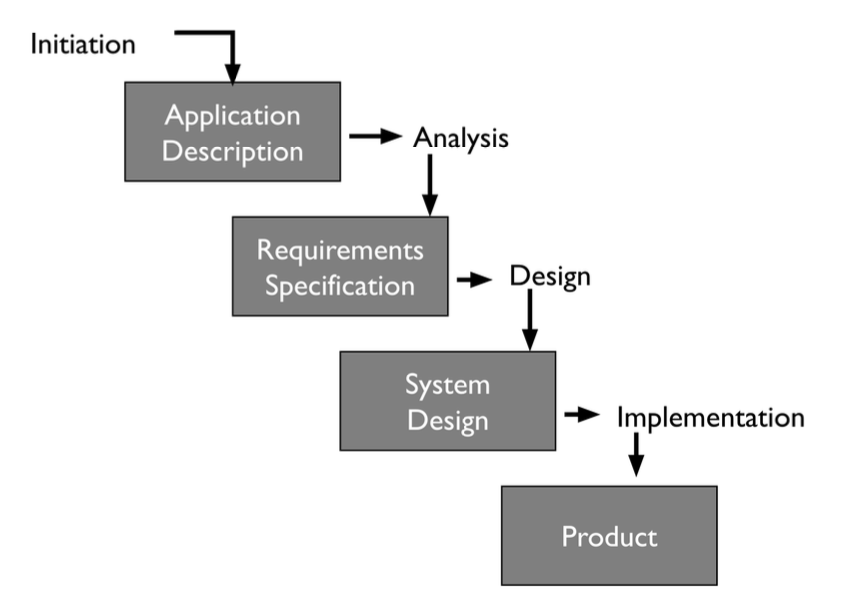
\includegraphics[width=0.8\textwidth]{waterfall.png}
  \caption{Waterfall design process}
\end{figure}

\begin{figure}[htbp]
  \centering
  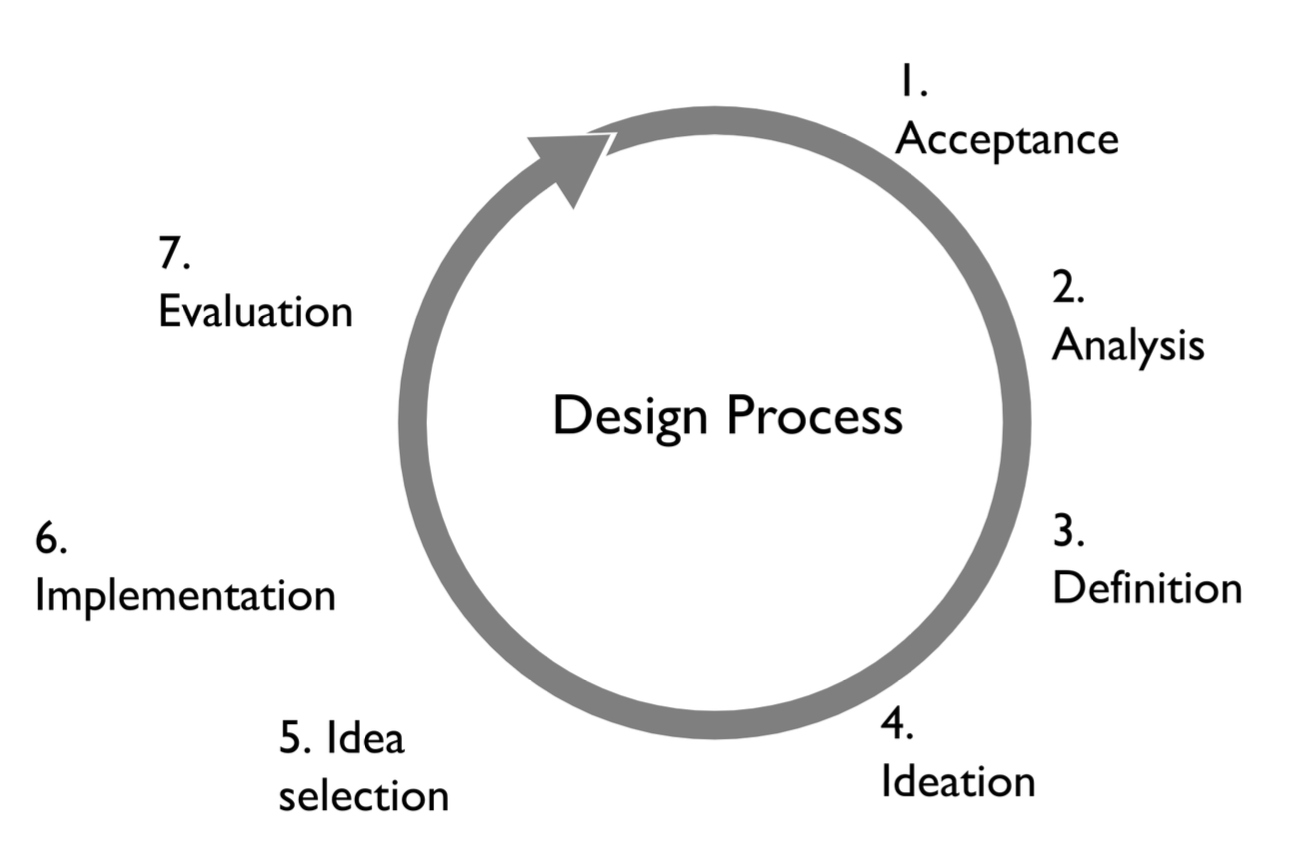
\includegraphics[width=0.8\textwidth]{agile.png}
  \caption{Agile design process, Koberg \& Bagnall}
\end{figure}

\begin{figure}[htbp]
  \centering
  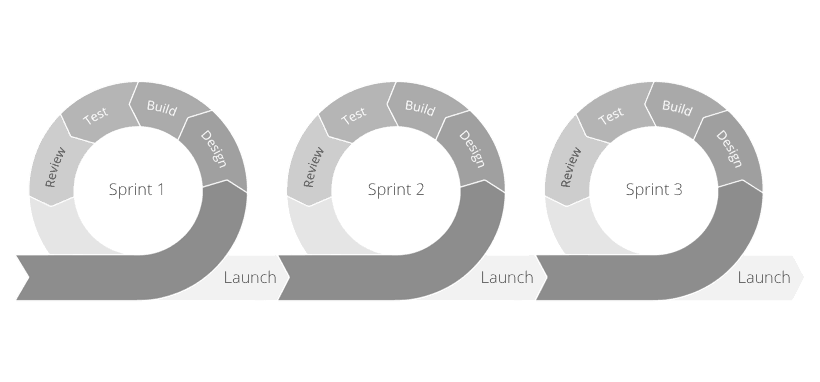
\includegraphics[width=0.8\textwidth]{agile-series.png}
  \caption{We may also model agile as a series of sprints}
\end{figure}

Waterfall is apparently cheaper, as it requires less revision work. This is true. It outputs a probabalistically insufficient solution at a reduced cost. Hence managerial types love it. Agile is more expensive. It's name, however, is in fashion. Hence managerial types love using it to describe their waterfall methodologies. Real agile is rare in practice, especially at larger firms where testing wuld mean literally getting test users together. For smaller startups, testing just means releasing a prototype to the public. Hence startups can more easily apply agile methods as they don't have a brand to protect from low fidelity prototypes being released to the public.

An excellent model for the number of ideas under consideration through agile, or cyclical design can be seen below. We see how divergent phases see the development of new potential solutions, followed by convergent phases, then testing, and with new problems identified, additional divergent ideas, until eventually a well-tested solution emerges. This is how startups build great products.

\begin{figure}[htbp]
  \centering
  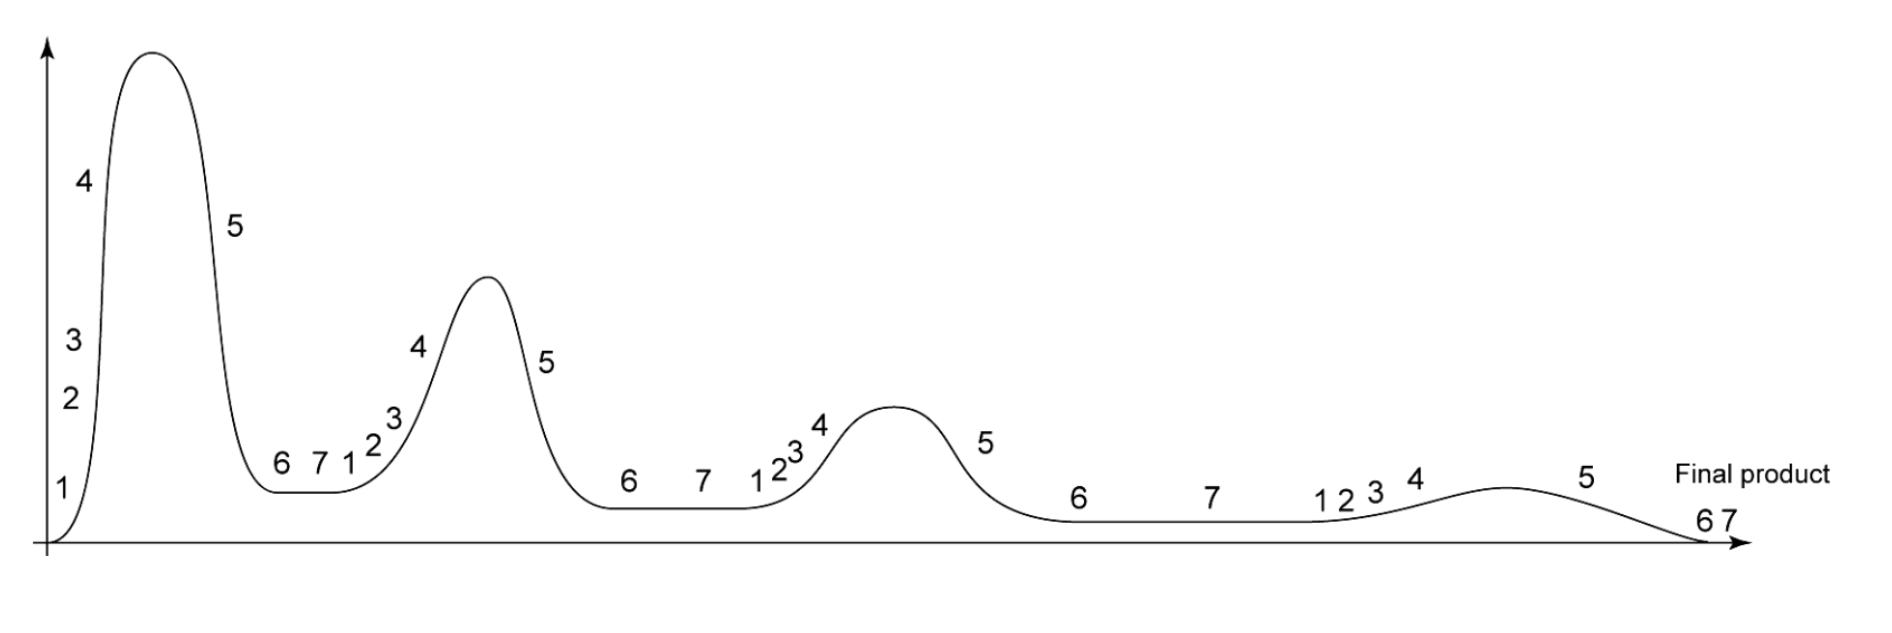
\includegraphics[width=0.8\textwidth]{ideas.png}
  \caption{The X axis is time, the Y axis is ideas under consideration. The numbers map to phases in the Koberg \& Bagnall design cycle in Figure 3.}
\end{figure}





\end{document}
